\documentclass[../TheoreticalMechanics.tex]{subfiles}

\begin{document}

\graphicspath{{HamiltonJacobiTheory/}}

\section{Hamilton-Jacobi理论} % (fold)
\label{sec:hamilton_jacobi理论}

\subsection{Hamilton-Jacobi方法} % (fold)
\label{sub:hamilton_jacobi方法}

\subsubsection{Hamilton-Jacobi方程} % (fold)
\label{ssub:hamilton_jacobi方程}

\begin{finale}
    \begin{theorem}[Hamilton-Jacobi方程]
        欲通过第二类变换$S=F_2\pare{q,P,t}$使新坐标系下的Hamilton量为零, 由\eqref{eq:正则变换下的Hamilton量},
        \[ H\pare{q_1,\cdots,q_n;\+D{q_1}DS,\cdots,\+D{q_n}DS;t} + \+DtDS = 0. \]
        其解谓Hamilton主函数. 其生成的变换使
    \end{theorem}
\end{finale}
\begin{remark}
    上述方程的解会有$n+1$个积分常数, 但其中一个以$S+\alpha$之形式出现, 故不影响$S$导出的变换.
\end{remark}
\begin{corollary}[Hamilton-Jacobi方程在两个坐标系下的解]
    设$\alpha_i$表示坐标$P_i$, 则$P_i$为常数, 且
    \[ Q_i = \beta_i = \+D{\alpha_i}D{S\pare{q,\alpha,t}},\quad p_i = \+D{q_i}D{S\pare{q,\alpha,t}}, \]
    可以通过求逆得到$q_j = q_j\pare{\alpha,\beta,t}$以及$p_j$.
\end{corollary}
\begin{corollary}[Hamilton主函数作为作用量]
    \label{coll:Hamilton主函数作为作用量}
    设$S$为Hamilton主函数, 则
    \[ \+dtdD = \+D{q_i}DS\dot{q}_i + \+DtDS = p_i\dot{q}_i - H = L. \]
    从而
    \[ S = \int L\,\rd{t} + \const. \]
\end{corollary}
\begin{corollary}[Hamilton特征函数]
    对于$H=a$守恒的情形, 存在$W$满足
    \[ S\pare{q,\alpha,t} = W\pare{q,\alpha} - at. \]
    其中$W$谓Hamilton主函数. 由\cref{coll:Hamilton主函数作为作用量},
    \[ p_i = \+D{q_i}DW, \quad \+dtdW = \+D{q_i}DW\dot{q}_i = p_i\dot{q}_i. \]
    从而
    \[ W = \int p_i\dot{q}_i\,\rd{t} = \int p_i\,\rd{q_i}. \]
\end{corollary}

% subsubsection hamilton_jacobi方程 (end)

\subsubsection{Hamilton-Jacobi方法的例子} % (fold)
\label{ssub:hamilton_jacobi方法的例子}

\begin{ex}
    一维谐振子的Hamilton-Jacobi方程为
    \[ \rec{2m}\brac{\pare{\+DqDS}^2 + m^2\omega^2q^2} + \+DtDS = 0 \Rightarrow \rec{2m}\brac{\pare{\+DqDW}^2 + m^2\omega^2q^2} = \alpha. \]
    其中$H=\alpha$是新的常量$P$坐标,
    \[ S = \sqrt{2m} \int \rd{q}\sqrt{\alpha-\frac{m\omega^2q^2}{2}} - \alpha t \Rightarrow \beta' = \+D\alpha DS = \sqrt{\frac{m}{2}}\int \frac{\rd{q}}{\sqrt{\alpha-\frac{m\omega^2q^2}{2}}} - t. \]
    \[ t+\beta' = \rec{\omega}\arcsin q\sqrt{\frac{m\omega^2}{2\alpha}}. \]
    \[ q = \sqrt{\frac{2\alpha}{m\omega^2}}\sin\pare{\omega t + \beta},\quad p = \+DqDS = \+DqDW = \sqrt{2m\alpha} \cos\pare{\omega t + \beta}. \]
    相应地可以通过$q_0$和$p_0$确定守恒量$\alpha$和$\beta$.
\end{ex}
\begin{lemma}[循环坐标在Hamilton特征函数中的项]
    设坐标变换后有循环坐标$\theta$及相应的动量$p_\theta$, 则相应的坐标在Hamilton特征函数中的项为
    \[ W_\theta = \theta\alpha_\theta. \]
\end{lemma}

% subsubsection hamilton_jacobi方法的例子 (end)

\subsubsection{Hamilton特征函数} % (fold)
\label{ssub:hamilton特征函数}

\begin{finale}
    \begin{theorem}[Hamilton-Jacobi方程对Hamilton特征函数的形式]
        Hamilton特征函数$W\pare{q,P}$满足
        \[ H\pare{q_i,\+D{q_i}DW} = \alpha_1, \]
        其中$\alpha_1$是经过由$W$生成的第二类变换变换后的一动量. $W$不含时, 故$\alpha_1=H=K$.
    \end{theorem}
\end{finale}
\begin{lemma}[Hamilton特征函数变换后坐标]
    \label{lem:Hamilton特征函数变换后坐标}
    经由$W$生成的第二类变换变换后的坐标有
    \[ \dot{P}_i = -\+D{Q_i}DK = 0, \quad \dot{Q}_i = \+D{\alpha_i}DK = \begin{cases}
        1,\quad i=1,\\
        0,\quad i\neq 1.
    \end{cases} \]
    这对于$Q_1$有
    \[ Q_1 = t+\beta_1 = \+D{\alpha_1}DW. \]
\end{lemma}
\begin{remark}
    Hamilton特征函数的Jacobi方程将时间参量单独分出, 便于求解轨道形状.
\end{remark}
\begin{longtable}{|c|c|c|}
    \hline
    性质 & $S$ & $W$ \\
    \hline
    Hamilton量 & $H\pare{q,p,t}$ & $H\pare{q,p}=\const$ \\
    \hline
    变换后坐标 & $Q_i,P_i$为常数 & $P_i$为常数 \\
    \hline
    $K$ & $K=0$ & 对所有坐标循环, $K=H=\alpha_1$ \\
    \hline
    $Q_i$ & $\beta_i$ & $Q_i = v_i t+\beta_i$ \\
    \hline
    $P_i$ & $\gamma_i$ & $\gamma_i$ \\
    \hline
    解 & $S\pare{q,P,t}$ & $W\pare{q,P}$ \\
    \hline
    \+:r2{方程} & \+:r2{$\displaystyle H\pare{q,\+DqDS,t}+\+DtDS=0$} & \+:r2{$\displaystyle H\pare{q,\+DqDW}-\alpha_1 = 0$} \\
    & & \\
    \hline
    积分常数 & $n$个积分常数 & $n-1$个非平凡积分常数, 以及$\alpha_1$ \\
    \hline
    其它动量 & \+:c2{c|}{总能选择新动量为$P_i = \gamma_i\pare{\alpha_1,\cdots,\alpha_n}$} \\
    \hline
    \+:r2{动量表示} & \+:r2{$\displaystyle p_i = \+D{q_i}DS$} & \+:r2{$\displaystyle p_i = \+D{q_i}DW$} \\
    & & \\
    \hline
    \+:r2{坐标表示} & \+:r2{$\displaystyle Q_i = \+D{\gamma_i}DS$} & \+:r2{$\displaystyle Q_i = \+D{\gamma_i}DW = v_i\pare{\gamma_j}t+\beta_i$} \\
    & & \\
    \hline
    $S$和$W$ & \+:c2{c|}{$S\pare{q,P,t}=W\pare{q,P} - \alpha_1 t.$} \\
    \hline
    \caption{$S$和$W$方法的对比}
\end{longtable}

% subsubsection hamilton特征函数 (end)

\subsubsection{分离变量} % (fold)
\label{ssub:分离变量}

\begin{definition}[完全可分的Hamilton主函数]
    Hamilton主函数谓完全可分的, 如果可以写为
    \[ S = \sum_i S_i\pare{q_i;\alpha_1,\cdots,\alpha_n;t} \]
\end{definition}
\begin{lemma}[Hamilton的分离常数]
    对于不含时的Hamilton, 有
    \[ S_i\pare{q_i;\alpha_q,\cdots,\alpha_n;t} - \alpha_i t \Rightarrow H_i\pare{q_i;\+D{q_i}D{W_i};\alpha_1,\cdots,\alpha_n} = \alpha_i. \]
    其中$\alpha_i$谓分离常数.
\end{lemma}

% subsubsection 分离变量 (end)

\subsubsection{Kepler问题} % (fold)
\label{ssub:kepler问题}

\begin{lemma}[有循环坐标的Hamilton特征函数]
    设$q_1$为循环坐标, 则可有$p_1=\gamma$,
    \[ W = W_1\pare{q_1,\alpha} + W'\pare{q_2,\cdots;q_n;\alpha} = \gamma q_1 + W'. \]
\end{lemma}
\begin{finale}
    \begin{theorem}[分离变量法]
        设$H$中含有$p_i, q_i$的项可以分离为$f\pare{q_j,p_j}$, $W$可分离为
        \[ W = W_j\pare{q_j,\alpha} + W'\pare{q_{i\neq j},\alpha}, \]
        则相应的
        \[ f\pare{q_j,\+D{q_j}D{W_j}} = \alpha_j = \const. \]
    \end{theorem}
\end{finale}
\begin{theorem}[St\"ackel条件]
    Hamilton-Jacobi方程是可分离变量的, 如果同时有
    \begin{cenum}
        \item Hamilton量是守恒的;
        \item $\displaystyle H = \half\brac{\+vp-\+va\pare{q}}\+vT^{-1}\ket{\+vp-\+va\pare{q}} + V\pare{q}$;
        \item $\displaystyle V\pare{q} = \sum_i \frac{V_i\pare{q_i}}{T_{ii}}$;
        \item 考虑同时成立
        \[ \pare{\phi^{-1}}_{ii} = \rec{T_{ii}},\quad \pare{\+D{q_i}D{W_i} - a_i} = 2\delta_{ik}\phi_{kj}\gamma_j \]
        的$\phi$, 其中$\gamma$是常矢量, 且$\phi_{ii}$和$\pare{\phi}^{-1}_{ii}$都仅是$q_i$的函数.
    \end{cenum}
\end{theorem}
\begin{corollary}[球坐标系下可分的条件]
    球坐标系下有
    \[ T_{rr} = m,\quad T_{\theta\theta} = mr^2,\quad T_{\phi\phi} = mr^2\sin^2\theta. \]
    欲使此时Hamilton-Jacobi方程可分, 需
    \[ V\pare{q} = V_r\pare{r} + \frac{V_\theta\pare{\theta}}{r^2} + \frac{V_\phi\pare{\phi}}{r^2\sin^2\theta}.  \]
\end{corollary}
\begin{ex}[中心力场问题]
    中心力场的Hamilton量为
    \[ H = \rec{2m}\pare{p_r^2 + \frac{p_\psi^2}{r^2}}+V\pare{r},\quad W = W_1\pare{r} + \alpha_\psi \psi. \]
    相应的Hamilton-Jacobi方程为
    \[ \pare{\+DrD{W_1}}^2 + \frac{\alpha_\psi^2}{r^2} + 2mV\pare{r} = 2m\alpha_1\Rightarrow W = \int\rd{r}\sqrt{2m\pare{\alpha_1-V}-\frac{\alpha_\psi^2}{r^2}}+\alpha_\psi\psi. \]
    由\cref{lem:Hamilton特征函数变换后坐标},
    \[ t+\beta_1 = \int \frac{m\,\rd{r}}{\sqrt{2m\pare{\alpha_1-V} - \frac{\alpha_\psi^2}{r^2}}}, \]
    \[ \beta_2 = \+D{\alpha_\psi}DW = -\int \frac{\alpha_\psi\,\rd{r}}{\sqrt{r^2\sqrt{2m\pare{\alpha_1 - V} - \frac{\alpha_\psi^2}{r^2}}}} + \psi. \]
\end{ex}
\begin{ex}[球坐标系下中心力场问题]
    \label{ex:球坐标系下中心力场问题}
    对球坐标系下的Hamilton-Jacobi方程分离变量, 即有
    \[ H = \rec{2m}\pare{p_r^2 + \frac{p_\theta^2}{r^2} + \frac{p_\phi^2}{r^2\sin^2\theta}} + V\pare{r} \]
    \[ \Rightarrow \pare{\+DrD{W_r}}^2 + \rec{r^2}\brac{\underbrace{\pare{\+D\theta D{W_\theta}}^2 + \frac{\alpha_\phi^2}{\sin^2\theta}}_{\alpha_\theta^2}} + 2mV\pare{r} = 2mE. \]
    同样做到了完全分离变量. 此处$\alpha_\phi$是角动量沿极轴的分量, 而$\alpha_\theta$是角动量.
\end{ex}

% subsubsection kepler问题 (end)

% subsection hamilton_jacobi方法 (end)

\subsection{作用量-角变量理论} % (fold)
\label{sub:作用量_角变量理论}

\subsubsection{单自由度的作用量-角变量理论} % (fold)
\label{ssub:单自由度的作用量_角变量理论}

\begin{definition}[周期运动的分类]
    周期运动若$\pare{q,p}$构成闭合曲线, 则谓之振动. $q$无界增加而$p$周期性振动, 则谓之转动.
\end{definition}
\begin{figure}[ht]
    \centering
    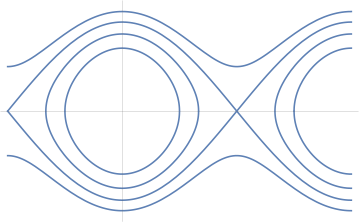
\includegraphics[width=6cm]{src/PendulumPhases.pdf}
    \caption{单摆在相空间中同时呈现振动和转动}
\end{figure}
\begin{theorem}[角变量]
    设
    \[ J = \oint p\,\rd{q}, \]
    有$\alpha_1 = H = H\pare{J}$, $W = W\pare{q,J}$, 又设$w$为与$J$共轭的坐标, 则
    \[ w = \+DJDW \Rightarrow \dot{w} = \+DJD{H\pare{J}} = \nu\pare{J} \Rightarrow w = \nu t+\beta. \]
    $w$谓角变量.
\end{theorem}
\begin{finale}
    \begin{theorem}[角变量与周期]
        $\Delta w$在一个周期内为
        \[ \Delta w = \oint \+DqDw\,\rd{q} = \oint \frac{\partial^2 W}{\partial q \partial J}\,\rd{q} = \+dJd{}\oint \+DqDW\,\rd{q} = \+dJd{}\oint p\,\rd{q} = 1. \]
        即$\Delta w = 1 = \nu\tau$.
    \end{theorem}
\end{finale}
\begin{ex}
    对于谐振子, 设$\alpha = E = H$, $\omega^2 = k/m$,
    \[ J = \oint p\,\rd{q} = \oint \sqrt{2m\alpha - m^2\omega^2q^2}\,\rd{q} = \frac{2\pi\alpha}{\omega} \Rightarrow \+DJDH = \frac{\omega}{2\pi} = \nu. \]
    特别地, 还可以发现$\pare{w,J}$到$\pare{q,p}$的变换为
    \[ q = \sqrt{\frac{J}{\pi m\omega}}\sin 2\pi w,\quad p = \sqrt{\frac{mJ\omega}{\pi}}\cos 2\pi w. \]
\end{ex}

% subsubsection 单自由度的作用量_角变量理论 (end)

\subsubsection{完全可分系统的作用量-角变量理论} % (fold)
\label{ssub:完全可分系统的作用量_角变量理论}

\begin{lemma}[可分系统的角变量]
    设系统完全可分, 则
    \begin{equation}
        \label{eq:可分系统的角变量共轭}
        J_i = \oint \+D{q_i}D{W_i\pare{q_i;\alpha_1,\cdots,\alpha_n}}\,\rd{q_i}, \quad W = \sum_j W_j\pare{q_j;J_1,\cdots,J_n}, 
    \end{equation}
    \begin{equation}
        \label{eq:角变量作为各个分量之和}
        \Rightarrow w_i = \+D{J_i}DW = \sum_{j=1}^n \+D{J_i}D{W_i\pare{q_j;J_1,\cdots,J_n}}, 
    \end{equation}
    \[ \Rightarrow \dot{w}_i = \+D{J_i}D{H\pare{J_1,\cdots,J_n}} = \nu_i\pare{J_1,\cdots,J_n}. \]
    \[ \omega_i = \nu_i t + \beta_i. \]
\end{lemma}
\begin{remark}
    循环坐标$q_i$相对的$p_i$为常量, 故$\pare{q,p}$图上为直线, 此时定义$J_i = 2\pi p_i$.
\end{remark}
\begin{lemma}[角变量对虚位移的变化]
    考虑独立的虚位移$\rd{q_j}$,
    \[ \delta w_i = \sum_j \+D{q_j}D{w_i}\,\rd{q_j} = \sum \frac{\partial^2 W}{\partial J_i\partial q_j}\,\rd{q_j} = \+D{J_i}D{}\sum_j p_j\pare{q_j,J}\,\rd{q_j}, \]
    \[ \Rightarrow \Delta w_i = \sum_j \+D{J_i}D{}\oint_{m_j}p_j\pare{q_j,J}\,\rd{q_j}. \Rightarrow \Delta\+vw = \+vm. \]
    其中$m_i$是坐标$q_i$所经周期数.
\end{lemma}
\begin{finale}
    \begin{lemma}[坐标对角变量的周期性]
        对于周期振动, $q_i$和$p_i$是角变量的周期(多)函数, 即任一$\omega_i$经过整数增加后必有$p_i$回复原值. 故
        \begin{equation}
            \label{eq:坐标对角变量的周期性}
            q_k\pare{t} = \sum_{\+vj\in\+bZ^n}a_{\+vj}^{\pare{k}}e^{2\pi \+vj\cdot\pare{\+v\nu t+\+v\beta}}, 
        \end{equation}
        其中
        \[ \+vw = \+v\nu t + \+v\beta. \]
        对于转动, 设$q_k$的坐标周期为$q_{0k}$, 则
        \[ q_k = q_{0k}\pare{v_k t + \beta_k} + \sum_{\+vj\in\+bZ^n}a_{\+vj}^{\pare{k}}e^{2\pi \+vj\cdot\pare{\+v\nu t+\+v\beta}}. \]
    \end{lemma}
\end{finale}
\begin{lemma}[角变量可分的情形]
    若\eqref{eq:角变量作为各个分量之和}简化为
    \[ w_i = \+D{J_i}D{w_i}\pare{q_i;J_1,\cdots,J_n}, \]
    则相应的\eqref{eq:坐标对角变量的周期性}简化为
    \[ q_k = \sum_j a_j^{\pare{k}}e^{2\pi ij w_k} = \sum_j a_j^{\pare{k}}e^{2\pi ij \pare{\nu_k t + \beta_k}}. \]
\end{lemma}
\begin{lemma}[$\pare{q,J}$到$\pare{q,w}$的变换]
    考虑
    \[ W' = W - \sum_k \omega_k J_k, w_k = \+D{J_k}D{W}. \]
    由\eqref{eq:可分系统的角变量共轭}, 当$\omega_k$增加$1$而其他量不变时, $W'$不变. 且$W'$生成一$\pare{q,J}$到$\pare{q,w}$的变换.
\end{lemma}
\begin{lemma}[退化频率约化角变量]
    \label{lem:退化频率约化角变量}
    设频率之间存在相关性, 即有$j_{ki}\in \+bZ$使得
    \[ \sum_{i=1}^n j_{ki}v_i = 0,\quad k = 1, \cdots, m. \]
    定义第二类的变换$\pare{w,J}\mapsto\pare{w',J'}$, 由
    \[ F_2 = \sum_{k=1}^m \sum_{i=1}^n J'_k j_{ki}w_i + \sum_{k=m+1}^n J'_k w_k \]
    生成, 则变换后坐标为
    \[ w'_k = \left\{\begin{array}{l}
        \sum_{i=1}^n j_{ki}w_i,\\
        w_k.
    \end{array}\right.\Rightarrow \nu'_k = \left\{\begin{array}{ll}
        \dot{w}'_k\sum_{i=1}^n j_{ki}\nu_i = 0, & k = 1,\cdots, m,\\
        \nu_k, & k = m+1,\cdots, n.
    \end{array}\right. \]
    \[ J_i = \sum_{k=1}^m J'_k j_{ki} + \sum_{k=m+1}^n J'_k\delta_{ki}. \]
\end{lemma}
\begin{lemma}[$H$无关于退化角变量]
    由
    \[ \nu'_i = \+D{J'_i}D{H}, \]
    若$\nu'_i=0$, 则$H$与$J'_i$无关.
\end{lemma}

% subsubsection 完全可分系统的作用量_角变量理论 (end)

\subsubsection{中心力场下的作用量-角变量理论} % (fold)
\label{ssub:中心力场下的作用量_角变量理论}

\begin{ex}
    \label{ex:中心力场问题下的角变量共轭}
    在\cref{ex:球坐标系下中心力场问题}中设定$V\pare{r} = -k/r$, 并借助\cref{ex:球坐标系下平方反比问题角变量积分}和\cref{ex:球坐标系下平方反比问题径向角变量积分}中的结论,
    \begin{align*}
        J_\phi &= \oint \+D\phi DW\,\rd{\phi} = \oint \alpha_\phi\,\rd{\phi} = 2\pi\alpha_\phi, \\
        J_\theta &= \oint \+D\theta DW\,\rd{\theta} = \oint \sqrt{\alpha_\theta^2 - \frac{\alpha_\phi^2}{\sin^2\theta}}\,\rd{\theta} = 2\pi\pare{\alpha_\theta-\alpha_\phi},\\
        J_r &= \oint \+DrDW\,\rd{r} = \oint \sqrt{2mE + \frac{2mk}{r} - \frac{\alpha_\theta^2}{r^2}}\,\rd{r} = -\pare{J_\theta + J_\phi} + \pi k\sqrt{\frac{2m}{-E}}.
    \end{align*}
\end{ex}
\begin{remark}
    可以发现$H$中唯一出现$J_\theta$和$J_\phi$的地方是离心势项, 这意味着频率存在退化, 这是因为运动一周后$\theta$和$\phi$都回复原值.
\end{remark}
\begin{theorem}[平方反比力场的退化频率]
    平方反比力场下,
    \[ H = E = -\frac{2\pi^2 mk^2}{\pare{J_r+J_\theta+J_\phi}^2}, \]
    故三个角变量频率皆相等,
    \[ v = \+D{J_r}D{H} = \+D{J_\theta}DH = \+D{J_\phi}DH \Rightarrow \tau = \pi k\sqrt{\frac{m}{-2E^3}}. \]
\end{theorem}
\begin{ex}
    将\cref{lem:退化频率约化角变量}应用到上述中心力场问题, 则
    \[ \begin{cases}
        v_\phi - v_\theta = 0,\\
        v_\theta - v_r = 0
    \end{cases} \Rightarrow F = \pare{w_\phi - w_\theta}J_1 + \pare{w_\theta - w_r}J_2 + w_rJ_3. \]
    \[ \begin{cases}
        w_1 = w_\phi - w_\theta,\\
        w_2 = w_\theta - w_r,\\
        w_3 = w_r,
    \end{cases}\quad \begin{cases}
        J_\phi = J_1,\\
        J_\theta = J_2 - J_1,\\
        J_r = J_3 - J_2,
    \end{cases}\Rightarrow \begin{cases}
        J_1 = J_\phi,\\
        J_2 = J_\phi + J_\theta,\\
        J_3 = J_\phi + J_\theta + J_r.
    \end{cases} \]
    \[ \Rightarrow H = -\frac{2\pi^2mk^2}{J_3^2}. \]
    注意$J_1$和$J_2$对应的频率退化, 只有$J_3$一个独立的频率.
\end{ex}
\begin{ex}
    应用\cref{thm:动能的变换}中的结论, 并应用「中心力场下的运动在同一平面上」之条件, 则
    \begin{equation}
        \label{eq:球坐标系下动能以动量表示}
        2T = p_r\dot{r} + p_\theta\dot{\theta} + p_\phi \dot{\phi} = p_r\dot{r} + p\dot{\psi}. 
    \end{equation}
    注意到$\phi$和$\psi$的周期相同, 可以据此重新计算\cref{ex:中心力场问题下的角变量共轭}中的
    \[ J_\theta = \oint p_\theta\,\rd{\theta} = \oint p\,\rd{\psi} - \oint p_\phi\,\rd{\phi}  = 2\pi\pare{p-p_\phi} = 2\pi\pare{\alpha_\theta - \alpha_\phi}. \]
\end{ex}
\begin{ex}[闭合轨道条件]
    由\cref{coll:幂势的位力定理}和\eqref{eq:球坐标系下动能以动量表示}, 在一个周期内有
    \[ -\frac{2H}{\nu_3} = J_r + J_\theta + J_\phi = J_3 \Rightarrow -\frac{2}{J_3} = \frac{v_3}{H} = \rec{H}\+d{J_3}dH \Rightarrow H = \frac{D}{J_3^2}. \]
    其中$D$仅与$m$与$k$有关. 考虑圆形轨道的情况下有
    \[ H = -\frac{k}{2r_0},\quad \frac{k}{r_0^2} = \frac{p^2}{mr_0^3} = \frac{J_3}{4\pi^2mr_0^3}. \]
    消除$r_0$可得(对椭圆轨道亦成立的)
    \[ H = -\frac{2\pi^2mk^2}{J_3^2}. \]
\end{ex}
\begin{ex}
    中心力场问题应当有$5$个守恒量. 分别是$J_1,J_2,J_3$与$w_1$和$w_2$, 因为后两者的频率为零. 这些量可以用更经典的守恒量表示.
    \[ J_2 = 2\pi\alpha_\theta = 2\pi l \Rightarrow J_1/J_2 = \cos \gamma. \]
    \[ a = -\frac{k}{2E} = \frac{J_3^2}{4\pi^2mk}. \]
    由\cref{thm:圆锥曲线轨道方程},
    \[ e = \sqrt{1-\frac{J_2^2}{4\pi^2mka}} = \sqrt{1-\pare{\frac{J_2}{J_3}}^2}. \]
    由\eqref{eq:可分系统的角变量共轭},
    \[ W = \int p_\phi\,\rd{\phi} + \int p_\theta\,\rd{\theta} + \int p_r\,\rd{r},\quad w_1 = \+D{J_1}DW. \]
    于是$w_1$右侧的求导只需对前两个积分进行.
    \[ p_\phi = \alpha_\phi = \frac{J_1}{2\pi},\quad p_\theta = \pm\sqrt{\alpha_\theta^2 - \frac{\alpha_\phi^2}{\sin^2\theta}} = \pm\rec{2\pi}\sqrt{J_2^2 - \frac{J_1^2}{\sin^2\theta}}. \]
    由\cref{ex:平方反比问题下第一角变量关联至普通守恒量的积分},
    \[ w_1 = \frac{\phi}{2\pi} + \frac{J_1}{2\pi}\int \frac{\rd{\theta}}{\sin^2\theta\sqrt{J_2^2 - J_1^2\csc^2\theta}}\Rightarrow 2\pi w_1 = \phi - u, \]
    其中$\sin u = \cot\gamma\cot\theta$, 故$u$即为质点在$\pare{x,y}$平面上的投影到中心的连线同「轨道与平面交点」之夹角. 从而$2\pi w_1$即为$x$轴与「轨道与平面交点」之夹角. 类似手段可得$2\pi w_2$是「轨道与平面交点」与近日点之间的夹角.
\end{ex}

% subsubsection 中心力场下的作用量_角变量理论 (end)

% subsection 作用量_角变量理论 (end)

% section hamilton_jacobi理论 (end)

\end{document}
